\documentclass[italian]{beamer}
%\documentclass[italian,handout]{beamer}

\usepackage[utf8]{inputenc}

% Uso un file unico, non serve molto

\title[Bitcoin]{Analisi di Bitcoin}
\subtitle{Anonimato, Sicurezza e Sviluppi Futuri}
\author[Paoluzzi Matteo]{Paoluzzi Matteo}
<<<<<<< local
\institute[UniUD]{Università degli Studi di Udine\and{}Relatore:\\{}Dott. Ivan Scagnetto}
=======
\institute[UniUD]{Università degli Studi di Udine\and{}Relatore:\\{}Prof. Ivan Scagnetto}
>>>>>>> other
\date[2014/04/03]{IV Sessione di Laurea AA 2012/2013, Aprile 2014}
\subject{Bitcoin}

\usepackage{default}
\usepackage{pres_commands}
%\usepackage{pres_uniudtesi}
\usetheme{Madrid}

\graphicspath{{./img/}}

\hypersetup{
  pdfstartview={Fit},
  pdftitle={Presentazione della Tesi ``Analisi di Bitcoin: Anonimato, Sicurezza e Sviluppi Futuri``},
  pdfauthor={Paoluzzi Matteo},
  pdfsubject={Modello di presentazione di Tesi al computer},
  pdfkeywords={LaTeX pdf presentazione tesi laurea}}

\begin{document}

\frame{\titlepage}

<<<<<<< local
\begin{frame}{Di cosa si tratta} % 1
Una valuta elettronica basata su crittografia a chiave pubblica progettata per:
=======
\begin{frame}{Di cosa si tratta}
>>>>>>> other
\begin{itemize}
<<<<<<< local
 \item Proteggere l'identità degli utenti sfruttando \textbf{indirizzi} anonimi.
 \item Essere indipendente da qualsiasi istituto di credito.
 \item Essere immune dal rischio di inflazione.
 \item Funzionare su base P2P in modo pubblico, sicuro e verificabile.
=======
 \item È una valuta utilizzabile per scambi commerciali.
 \item Esiste solo in forma elettronica.
 \item Non ha confini geografici.
 \item Bitcoin indica la rete e il protocollo.
 \item L'unità monetaria si indica con BTC.
>>>>>>> other
\end{itemize}
\end{frame}

<<<<<<< local
\begin{frame}{Indirizzi} % 2
L'anonimato dell'utente viene implementato tramite stringhe di testo note come indirizzi.
=======
\begin{frame}{Criteri di progettazione}
>>>>>>> other
\begin{itemize}
<<<<<<< local
 \item Un indirizzo viene generato a partire da una coppia di chiavi pubbliche e private.
 \item Tutte le \textbf{transazioni} di BTC avvengono da e verso indirizzi, senza divulgare informazioni sull'identità delle parti coinvolte.
 \item Le chiavi di cifratura consentono di spendere il denaro ricevuto e impedire che il denaro inviato finisca ad un destinatario diverso da quello desiderato.
 \item Ogni utente è incoraggiato ad avere molteplici indirizzi, mantenendo sicure le porzioni private delle chiavi appositamente generate.
=======
 \item Struttura completamente decentralizzata formata da nodi in un grafo casuale.
 \item Anonimato dell'utente.
 \item Indipendente da istituti centrali.
 \item Transazioni sicure e verificabili.
>>>>>>> other
\end{itemize}
\end{frame}

<<<<<<< local
\begin{frame}{Transazioni} % 3
Contengono tutte le informazioni necessarie per effettuare un ''trasferimento`` di denaro.
=======
\begin{frame}{Implementazione}
>>>>>>> other
\begin{itemize}
<<<<<<< local
 \item Sono identificate da un hash calcolato su un suo sottoinsieme di dati che ne cristallizzano le proprietà più rilevanti.
 \item Contengono molteplici sezioni di input e output costituite da script eseguibili che autorizzano la spesa e determinano l'invio del denaro:
=======
 \item Si usa la cifratura a chiave pubblica per creare una serie di indirizzi in cui verrà depositato il denaro.
 \item Ogni transazione viene firmata con la chiave privata del mittente e contiene la chiave pubblica del destinatario.
>>>>>>> other
 \begin{itemize}
<<<<<<< local
  \item L'input contiene un riferimento ad output di precedenti transazioni da cui prelevare denaro, e per ogni riferimento la chiave pubblica del creatore della transazione attuale e la relativa firma ECDSA che ne autorizzano il prelievo.
  \item Ogni output contiene un ammontare in denaro e uno script con l'indirizzo del destinatario che autorizzerà future spese della transazione.
  \item Se l'input è maggiore dell'output, il resto viene inviato ad un indirizzo scelto dal creatore della transazione.
=======
    \item Solo il destinatario di una transazione può spendere il denaro trasferito come unico proprietario della chiave privata richiesta.
    \item Si viene a creare una catena di transazioni legate dalle chiavi pubbliche e private di mittente e destinatario.
>>>>>>> other
 \end{itemize}
<<<<<<< local
=======
 \item Tutte le transazioni vengono rese pubbliche e confrontate tra loro in modo che nessuno possa spendere lo stesso denaro due volte.
 \item Le transazioni vengono fissate in blocchi che vengono concatenati tra loro.
>>>>>>> other
\end{itemize}
\end{frame}

<<<<<<< local
\begin{frame}{Blocchi} % 4
Le transazioni vengono raccolte in un blocco calcolando un hash il cui valore non deve superare un determinato target:
=======
\begin{frame}{Sicurezza: le transazioni}
>>>>>>> other
\begin{itemize}
<<<<<<< local
 \item Trovare tale hash è un lavoro computazionalmente molto difficile chiamato \textbf{mining} e viene mantenuto tale ridimensionando il target ogni 2016 blocchi in modo da generare in media un blocco ogni 10 minuti.
 \item Il nodo che trova il blocco viene premiato con una cifra fissa di BTC e con alcune tariffe prelevate dalle transazioni contenute nel blocco appena trovato e stabilite dal creatore delle transazioni in questione.
=======
    \item L'input di una transazione può solo essere l'output di una precedente transazione.
    \item Non è possibile spendere denaro che non è stato inviato ad un indirizzo di cui non si possiede la chiave privata.
    \item Le transazioni sono bloccate nel tempo da un timestamp e da un hash che le identifica in modo permanente.
    \item La rete verifica che uno stesso input non sia stato inviato a diversi output: un tentativo di attacco doppia-spesa.
>>>>>>> other
\end{itemize}
<<<<<<< local
Dato che ogni blocco contiene l'hash del blocco precedente, nell'insieme formano una \textbf{blockchain} il cui scopo è fissare le transazioni nel tempo in modo che non possano essere arbitrariamente modificate, garantendo così la sicurezza della rete e il buon esito delle transazioni.
=======
>>>>>>> other
\end{frame}

<<<<<<< local
\framedgraphic{Infografica}{transactions_ABC} % 5
=======
\begin{frame}{Sicurezza: i blocchi}
I blocchi vengono creati risolvendo un difficile problema crittografico.
\begin{itemize}
  \item Trovare l'hash di alcuni dati in modo che risulti un valore esadecimale inferiore ad uno specifico target.
  \item Il target viene ricalcolato ogni 2016 blocchi mantenendo fisso a 10 minuti il tempo medio per trovare un blocco.
  \item Tra i dati di cui calcolare l'hash ci sono le transazioni e l'hash del blocco precedente.
  \begin{itemize}
    \item La modifica di un blocco richiede la modifica di tutti i blocchi successivi.
    \item Concatenare blocchi rende sempre più difficile modificare un blocco vecchio.
    \item La catena di blocchi usata per fissare tutte le transazioni prende il nome di Blockchain.
  \end{itemize}
\end{itemize}
\end{frame}
>>>>>>> other

<<<<<<< local
\begin{frame}{Vulnerabilità: velocità di transazioni} % 6
=======
\framedgraphic{Infografica}{transactions_ABC}

\begin{frame}{Vulnerabilità: velocità di transazioni}
>>>>>>> other
 \begin{itemize}
  \item Un transazione non è confermata fintanto che non viene inserita in un blocco, il che richiede in media 10 minuti.
  \item Una transazione non confermata potrebbe non essere inserita nella blockchain e quindi risultare scartata.
  \item Un attacco doppia-spesa sfrutta questa debolezza per frodare un venditore poco accorto: \pause
  \begin{enumerate}
   \item Si crea una transazione legittima e la si invia al commerciante. \pause
   \item Il commerciante si fida che la transazione vada bene e invia il prodotto all'attaccante. \pause
   \item L'attaccante invia una seconda transazione che sovrascrive la prima inviando lo stesso denaro a se stesso, frodando il commerciante. \pause
   \item Se la seconda transazione viene inserita in un blocco prima della transazione legittima, l'attacco ha successo e l'attaccante ha ottenuto un bene senza pagarlo.
  \end{enumerate}
 \end{itemize}
 \pause
 La prevenzione è sempre nelle mani dell'utente.
\end{frame}

<<<<<<< local
\begin{frame}{Vulnerabilità: potenza di calcolo} % 7
=======
\begin{frame}{Vulnerabilità: potenza di calcolo}
>>>>>>> other
 Se un utente riesce ad accumulare più potenza di calcolo di quella del resto della rete, potrebbe creare una nuova blockchain a sua discrezioni invalidando tutte le transazioni a partire da un momento a sua discrezione.\\
 \bigskip
 \pause
 La difficoltà nel compiere tale operazione è elevata.
 \bigskip
 \pause
 Ma questo non vuol dire che sia impossibile!
\end{frame}

<<<<<<< local
\begin{frame}{Privacy} % 8
Il sistema di indirizzi adottato è simile a quello dei conti bancari in Svizzera: numeri di conto non collegabili direttamente a persone.\\
Ma il sistema di cifratura a chiave pubblica permette di aggregare indirizzi appartenenti alla stessa persona:
=======

\begin{frame}{Mining}
Creare un blocco ha molteplici scopi.
\pause
>>>>>>> other
\begin{itemize}
<<<<<<< local
 \item Una transazione contenente più indirizzi in input indica che tali indirizzi appartengono tutti al creatore della transazione stessa.
 \item Se una transazione contiene un output molto piccolo e destinato ad un indirizzo mai visto prima, probabilmente tale indirizzo è stato creato appositamente dal creatore della transazione per raccogliere il resto.
=======
  \item Blocca le transazioni in modo permanente.
  \item Permette la creazione di nuova moneta.
  \begin{itemize}
    \item Il lavoro speso per trovare il blocco viene ricompensato con BTC create ``dal nulla''.
    \item Il numero di BTC si dimezza ogni 210000 blocchi per mantenere il numero massimo di BTC a circa 21 milioni.
    \item Inizialmente il premio era di 50 BTC, ora è sceso a 25 BTC.
  \end{itemize}
>>>>>>> other
\end{itemize}
<<<<<<< local
Creando un grafo delle transazioni pubblicamente disponibile e applicando le aggregazioni descritte, è possibile creare un secondo grafo approssimato rappresentante il flusso di monete tra utenti invece che tra indirizzi. Unendo questi due grafi ad altre fonti esterne potrebbe essere possibile identificare effettivamente un utente e tracciarne le attività.
=======
\bigskip
\pause L'analogia è con i cercatori d'oro, che guadagnano dal ritrovamento delle pepite dopo ore di duro lavoro in miniera. \\
\pause Pertanto il processo di calcolo dell'hash di un nuovo blocco viene definito \emph{mining} e il nodo \emph{miner}.
>>>>>>> other
\end{frame}

<<<<<<< local
\begin{frame}{Esempio reale: un furto} % 9
Il 13 Giugno 2011 sembra sia avvenuto un furto di circa 25000 BTC.\\
Analizzando il flusso delle transazioni si è potuto osservare come il furto abbia coinvolto più di 34100 indirizzi, alcuni mai visti prima ed altri appartenenti a entità note come il gruppo hacker LulzSec (non associabile al furto) e il servizio MyBitcoin.\\
Sfruttando le tecniche descritte è stato possibile unificare più indirizzi diversi ad una stessa entità, dimostrando quindi come sia possibile minacciare la privacy di un utente aggregando le informazioni disponibili online e offline.
=======
\begin{frame}{Mining Pools}
  Calcolare l'hash per un blocco è un evento casuale senza memoria che richiede elevata potenza di calcolo per essere portato a termine in tempi rapidi.
 \begin{itemize}
  \item Un computer end-user ha decisamente poche speranze di trovare un blocco e intascare la ricompensa.
  \item Con del costoso hardware dedicato le speranze aumentano un poco, ma restano comunque basse.
 \end{itemize}
 \bigskip
 \pause La soluzione è una collaborazione tra gli utenti in quelle che vengono definite \emph{mining pools}.
>>>>>>> other
\end{frame}

<<<<<<< local
\begin{frame}{Seguire le transazioni} % 10
\begin{figure}[htbp]
\centering
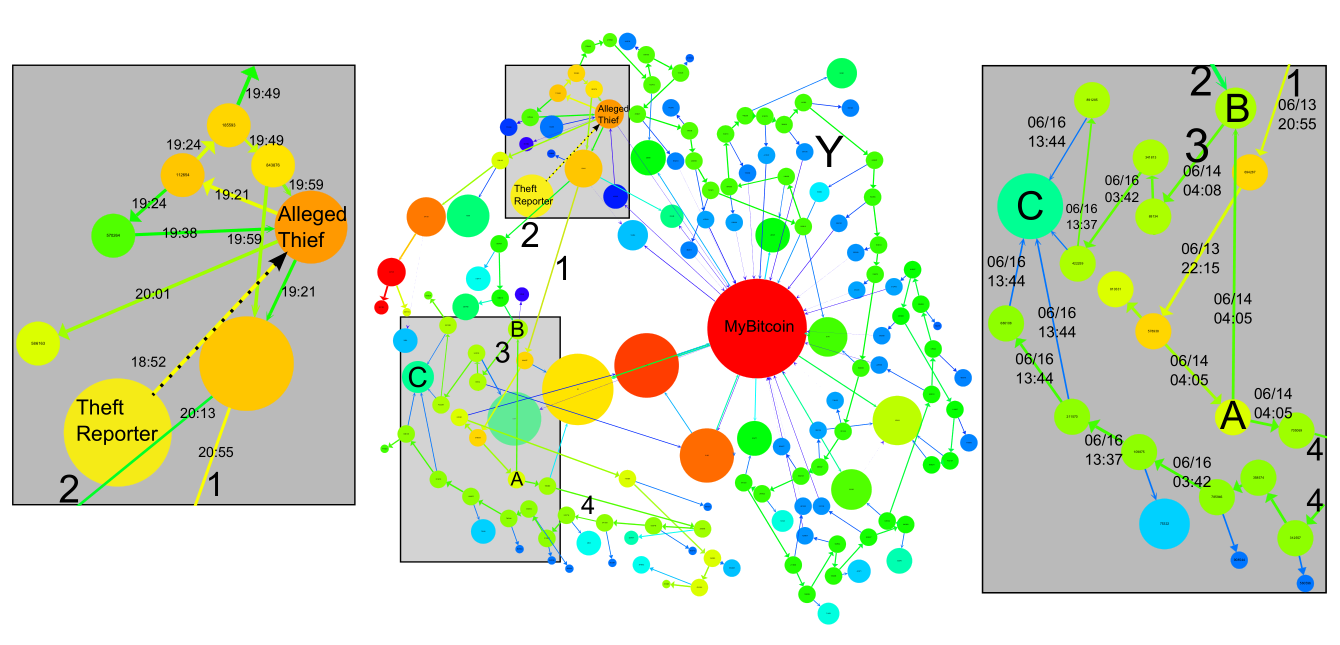
\includegraphics[width=\textwidth]{anonimato_1_13.PNG}
\end{figure}
=======
\begin{frame}{Mining Pools}
  Mantenendo l'analogia con i minatori, le mining pools sono compagnie minerarie.
 \begin{itemize}
  \item Più minatori si cimentano in contemporanea nel ritrovamento di un blocco.
  \item Ad ogni blocco trovato la ricompensa viene divisa tra tutti coloro che hanno collaborato.
  \item Ogni pool ha un suo sistema di retribuzione con i suoi vantaggi e svantaggi.
 \end{itemize}
>>>>>>> other
\end{frame}

<<<<<<< local
=======
\begin{frame}{Scripting}
Il protocollo sfrutta un linguaggio di scripting che permette di verificare le transazioni ma anche di crearne alcune che implementano situazioni diverse dal semplice pagamento.
\begin{itemize}
\item Sistemi di deposito temporaneo.
\item Raccolte fondi con assicurazione.
\item Acquisto di beni con un mediatore.
\end{itemize}
\bigskip
\pause
Essendo non-standard, attualmente queste transazioni vengono rifiutate dai nodi e non possono entrare a far parte della blockchain.\\
Possono però essere usare in reti private con client ad-hoc.
\end{frame}

\begin{frame}{Deflazione}
 L'elevato valore tendenzialmente crescente di una singola BTC rende più attraente l'idea di accumularle invece che di spenderle. Questo è vero per almeno il 55\% delle BTC prodotte. L'accumulazione di BTC provoca la seguente catena di eventi:
 \begin{enumerate}
  \item Meno transazioni. \pause
  \item Meno blocchi nell'unità di tempo. \pause
  \item Meno nuove monete. \pause
  \item Meno motivazione a diventare miner. \pause
  \item Meno utenti che verificano la correttezza delle transazioni. \pause
  \item Maggiore debolezza ai devastanti attacchi basati su potenza di calcolo e verifiche di transazioni. \pause
 \end{enumerate}
 Bitcoin è fortemente dipendente da una comunità attiva e da un costante fluire della moneta: in mancanza di ciò, perde il suo valore avviando potenzialmente una spirale deflazionistica.
\end{frame}

\begin{frame}{Questioni Legali}
  Data la sua natura volutamente ambigua, dal punto di vista legale ancora molto poco è stato definito per Bitcoin, e solo in ambiti limitati.\pause
  \begin{itemize}
   \item Le Bitcoin sono una forma di valuta? \pause
   \item Come verifico la proprietà di un oggetto acquistato con BTC in mancaza di ricevuta?\pause
   \item Sotto quale giurisdizione ricadono le BTC? \pause
   \item Come risolvo il problema del riciclaggio di denaro? \pause
   \item Sono un bene da tutelare?\pause
   \begin{itemize}
    \item Come identifico un eventuale ladro se è tutto anonimo? \pause
    \item Come calcolo le tasse, ammesso che debba calcolarle? \pause
    \item Come gestisco le eredità in caso di portafogli cifrati e mancanza di chiave privata?
   \end{itemize}
  \end{itemize}
\end{frame}

\begin{frame}{Litecoin ed altre}
  Creata nel 2011, è una variante di Bitcoin che sta avendo notevole diffusione:
  \begin{itemize}
   \item Un blocco ogni 2.5 minuti.
   \item 84 milioni di LTC.
   \item Ricompensa dimezzata ogni 840000 blocchi.
  \end{itemize}
  Esistono moltre altre monete elettroniche... \pause
  \begin{itemize}
    \item $\ldots$ alcune diffuse come Namecoin, PPCoin e Mastercoin $\ldots$ \pause
    \item $\ldots$ altre meno note come Megacoin e Anoncoin $\ldots$ \pause
    \item $\ldots$ e altre ancora umoristiche create apposta per farsi quattro risate, come Dogecoin e Coinye $\ldots$ \pause
  \end{itemize}
  $\ldots$ Ma tutte basate sugli stessi principi di decentralizzazione e anonimato e tutte perfettamente ``funzionanti''.
\end{frame}
>>>>>>> other



%%%%%%%%%%%%%%%%%%%%%%%%%%%%%%%%%%%%%%%%%%%%%%%%%%%%%%%%%%%%%%%%%%%%%%%%%%%%%%%%%%%%
% \item Formula che appare un poco per volta:
% \pause
% \parstepwise{
% $$
%   1\step{{}+2}
%   \step{{}+3} \step{{}+4}\step{{}+\cdots+n}
%   \step{{}={}}
%   \step{\sfondogiallo{$\displaystyle\frac{n(n+1)}{2}$}}
% $$
% }
%
%\pageTransitionGlitter{0}
% il comando \newframe e' come \newpage,
% ma non avanza il numero di pagina.
% Puo' servire per fare cambiamenti incrementali
% a una pagina, quando \pause o \stepwise non
% bastano. In questo esempio \pause non va bene
% perche' qui bisogna aggiungere un paragrafo
% ma allo stesso tempo  cambiare la figura che
% sta in cima alla pagina. Macchinoso da scrivere,
% ma puo' valerne la pena.
%
%\newframe
%
%\sfondogiallo{\rosso{\textit{coincidono:}}}
%
% Le transizioni si attivano al /pause
%\pageTransitionWipe{0}
%\pageTransitionWipe{180}
%\pageTransitionSplitVO
%\item {\setlength{\baselineskip}{2\baselineskip}
%Vedere la documentazione del pacchetto \textcolor{darkorange}{\texttt{texpower}}.
%}
%\pageTransitionReplace
%\pageTransitionBoxI
%%%%%%%%%%%%%%%%%%%%%%%%%%%%%%%%%%%%%%%%%%%%%%%%%%%%%%%%%%%%%%%%%%%%%%%%%%%%%%%%%%%%
\end{document}
